% !TeX root = ./Skript_DB.tex
\cohead{\Large\textbf{Grundlagen ERM}}
\section[Enity-Relationship-Modell]{Enity-Relationship-Modell}
\subsection[Datenbanken]{Datenbanken - Einführung}
Datenbanken enthalten, wie der Name schon sagt, große Mengen an Daten, z.B. eine Firma, die ihre Kunden mit Anschrift und die zugehörigen Bestellungen speichern muss. Das Verwalten und Durchsuchen von großen Mengen an Daten ist nicht trivial, z.B. würde Excel schnell an seine Grenzen stoßen, wenn z.B. eine Firma ihre Produkte, Kunden, Bestellungen, usw. speichern will. Datenbanken wurden genau zu diesem Zweck, dem Speichern und Bearbeiten von großen Mengen an Daten entwickelt.

Die Daten sollen übersichtlich gespeichert werden und so, dass man sie bearbeiten und durchsuchen kann. Dafür benötigt man eine Struktur. Stellen wir uns vor, eine Firma würde alle Daten, also Bestellungen, Kundendaten, Produktbeschreibungen, Preise, Rechnungen, Daten zu Angestellten, usw. einfach ausdrucken und in einen riesigen Container zusammen werfen. Die Daten wären zwar vorhanden, aber sucht man nun nach der Bestellung von John Wick, weil er sich beschwert, einen Toaster statt eines Eierkochers bekommen zu haben, so würde dies exorbitant viel Zeit in Anspruch nehmen. Würde man jedoch alle Bestellungen zusammen in einem Ordner sammeln, wäre die Suche deutlich einfacher. Die Daten sind dann strukturiert und damit übersichtlicher und einfacher zu bearbeiten. Etwas Ähnliches macht man auch mit den Daten in einer Datenbank. Sehr häufig wird das Enity-Relationship-Modell (ERM) verwendet, um die Daten zu strukturieren.
\subsection[Grundlagen]{Enity-Relationship-Modell}
Das Enity-Relationship-Modell (ERM) dient dazu die Struktur von Daten darzustellen, z.B., dass ein Kunde über einen Namen, Vornamen und eine Adresse verfügt. Wie genau ein bestimmter Kunde heißt oder wo er wohnt spielt für das ERM keine Rolle. Dazu wird eine Grafik, das ER-Diagramm angefertigt sowie eine Beschreibung der Elemente dieser Grafik. In unseren Beispielen werden die Elemente selbsterklärend sein und wir werden uns die Beschreibung sparen (Im obigen Beispiel ist klar, was Name, Vorname und Adresse des Kunden sind. Es ist keine zusätzliche Beschreibung notwendig).

Für die grafische Darstellungen werden wir die \texttt{Chen-Notation} verwenden. Die wesentlichen Elemente eines ERMs sind:
\begin{tcolorbox}[title=Entitätstypen und Entitäten]
	Darstellung eines meistens in der Realität vorhandenen Objekts auf der Datenbank, z.B. Kunde, Schüler oder Rechnung. Der Entitätstyp ist die abstrakte Darstellung, z.B. Schüler, während eine Entität eine konkrete Ausprägung, also ein Beispiel ist. So wäre der Schüler Momen Subotic eine Entität in der Datenbank.
	Weitere Beispiele für Entitäten sind:
	\begin{itemize}
		\item Individuen: Person Heinrich Müller, Firma GehtganzGut, Kunde Maria Meyer
		\item Konkreter Gegenstand: Raum A-308, Abteilung Lohn\&Gehalt, Wohnort Berlin
		\item Ereignis: Buchung, Mahnung, Vermietung
		\item Abstraktes: Unterricht, Klasse, Zahlungsart, Tagesplan
	\end{itemize}
	Eine Entität ist immer Mitglied einer Gruppe, des Entitätstyps. Diese kategorisiert also Entitäten mit gleichen Eigenschaften. So sind z.B. die Schülerin Christine Adler und der Schüler Christopher Jäger konkrete individuell identifizierbare Objekte, zu denen Informationen gespeichert werden. Da sie aber die gleichen Eigenschaften haben, gehören sie zum Entitätstyp Schüler. Welche Objekte so wichtig sind, dass sie als Entitätstyp in das Datenbankmodell aufgenommen werden sollen, muss sich an den funktionellen und informatorischen Zusammenhängen der zu speichernden Daten orientieren.
	Der Entitätstyp, also die Menge der Entitäten, wird in der grafischen Darstellung des ER-Modells, dem ER-Diagramm, als Rechteck dargestellt und die Bezeichnung eines Entitätstyps ist immer ein Substantiv.
\end{tcolorbox}
\begin{tcolorbox}[title=Beziehungen]
	Verknüpfungen von Entitäten, z.B. ist eine Rechnung immer einem bestimmten Kunden zugeordnet. Oft kann ein Entitätstyp Beziehungen zu vielen anderen Entitätstypen haben. So könnte die Rechnung nicht nur mit einem Kunden, sondern auch mit dem Entitätstyp Produkt verknüpft sein, der die bestellten Waren angibt.

	Durch Beziehungen werden die Wechselwirkungen oder Abhängigkeiten von Entitäten ausgedrückt. Beziehungen können ebenfalls Attribute (Eigenschaften) besitzen. Ein Beziehungstyp ist, analog zum Entitätstyp, die Abstraktion gleichartiger Beziehungen. Die Beziehung wird dabei meist durch Verben beschrieben und soll in Beziehungsrichtung einen vollständigen Satz ergeben.

	Beispiele für Beziehungen:
	\begin{itemize}
		\item Kind gehört zu Eltern
		\item Team verfügt über Betreuer
		\item Team besteht aus Teammitglied
	\end{itemize}
	Der Beziehungstyp wird grafisch durch eine Raute dargestellt, die durch zwei Kanten mit den Entitätstypen verbunden ist. In der Raute steht der Name des Beziehungstyps.
\end{tcolorbox}
\begin{tcolorbox}[title=Attribute]
	Attribute, auch als Eigenschaft oder Merkmal bezeichnet, beschreiben die Entitäten näher. Alle Entitäten eines Entitätstyps besitzen dieselben Attribute, jedoch sind die Attributswerte unterschiedlich. Attribute charakterisieren also eine Entität, einen Entitätstyp, eine Beziehung bzw. einen Beziehungstyp.

	Beispiele für Attribute:
	\begin{itemize}
		\item Name, Vorname oder Adresse einer Person
		\item Betrag einer Rechnung oder Bestellung
		\item Klassengröße oder Klassenzimmer einer Klasse
	\end{itemize}
	In der grafischen Darstellung werden Attribute als Ellipsen oder Kreise dargestellt. Diese sind über ungerichtete Kanten mit dem Entitätstyp verbunden.
\end{tcolorbox}
\begin{minipage}{\textwidth}
	\begin{minipage}{0.33\textwidth}
		\centering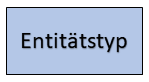
\includegraphics[width=4cm]{\pics/ERMEntity.png}

		Grafische Darstellung eines Entitätstyps.
	\end{minipage}
	\begin{minipage}{0.33\textwidth}
		\centering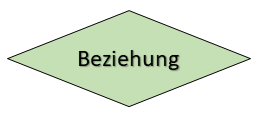
\includegraphics[width=4cm]{\pics/ERMRelationship.png}

		Grafische Darstellung einer Beziehung.
	\end{minipage}
	\begin{minipage}{0.33\textwidth}
		\centering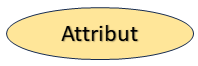
\includegraphics[width=4cm]{\pics/ERMAttribute.png}

		Grafische Darstellung eines Attributs.
	\end{minipage}
\end{minipage}
\begin{Exercise}[title={Beantworte folgende Fragen.}, label=ERMFragen1]
	\begin{enumerate}
		\item Worin liegt der Unterschied zwischen Entitäten und Entitätstypen?
		\item Worin liegt der Unterschied zwischen Attributen und Attributswerten?
	\end{enumerate}
\end{Exercise}
%%%%%%%%%%%%%%%%%%%%%%%%%%%%%%%%%%%%%%%%%
\begin{Answer}[ref=ERMFragen1]
	\begin{enumerate}
		\item Worin liegt der Unterschied zwischen Entitäten und Entitätstypen?

		Ein Entitätstyp ist der abstrakte Übergriff, z.B. Schüler, während eine Entität ein konkretes Beispiel ist, z.B. der Schüler Noah Schimek ist eine Entität vom Entitätstyp Schüler.
		\item Worin liegt der Unterschied zwischen Attributen und Attributswerten?

		Auch hier ist das Attribut die abstrakte Eigenschaft, z.B. hat der Entitätstyp Schüler ein Attribut Namen. Den Wert eines Attributs erhält man, wenn man eine bestimmte Entität betrachtet, z.B. hat das Attribut Namen beim obigen Schüler den Wert Noah Schimek.
	\end{enumerate}
\end{Answer}
\begin{Exercise}[title={Erstelle jeweils ein ERM}, label=ERMErstellen1]
	\begin{enumerate}
		\item Ein Fahrradverleih am Bodensee verleiht Damen-, Herren- und Kinderfahrräder. Dabei wird für jedes Fahrrad ein eigener Mietvertrag abgeschlossen. Eine Person kann mehrere Fahrräder mieten. Der Fahrradverleih möchte eine Datenbank aufbauen. Helfen Sie dabei.
		\item Ein befreundeter Autohändler bittet uns beim Aufbau einer Kundendatenbank zu helfen. Zuerst soll diese in einem ERM modelliert werden. Darin erscheinen sollen Kunde, Auto, Karosserietyp und Reifen. Ein Auto gehört dabei zu einem Kunden, ein Kunde kann aber mehrere Autos haben.
		\item Ein DVD-Verleiher betreibt mehrere Filialen (id, strasse, plz), wo es jeweils mehrere Medien (DVDs, BluRays, Spiele) zu leihen gibt. Jeder Kunde kann nur einer Filiale zugeordnet sein. Jeder Kunde kann mehrere Medien ausleihen. Ein Mitarbeiter kann nur in einer Filiale arbeiten.
	\end{enumerate}
\end{Exercise}
%%%%%%%%%%%%%%%%%%%%%%%%%%%%%%%%%%%%%%%%%
\begin{Answer}[ref=ERMErstellen1]
	Anmerkung: Die ERMs sind nur Lösungsvorschläge. Man kann auch zusätzliche Attribute hinzufügen. Zudem sind die ERMs nicht vollständig, wir werden später noch neue Begriffe kennen lernen, die hier noch fehlen.
	\begin{enumerate}
		\item Ein Fahrradverleih am Bodensee verleiht Damen-, Herren- und Kinderfahrräder. Dabei wird für jedes Fahrrad ein eigener Mietvertrag abgeschlossen. Eine Person kann mehrere Fahrräder mieten. Der Fahrradverleih möchte eine Datenbank aufbauen. Helfen Sie dabei.

		\begin{minipage}{0.8\textwidth}
			\centering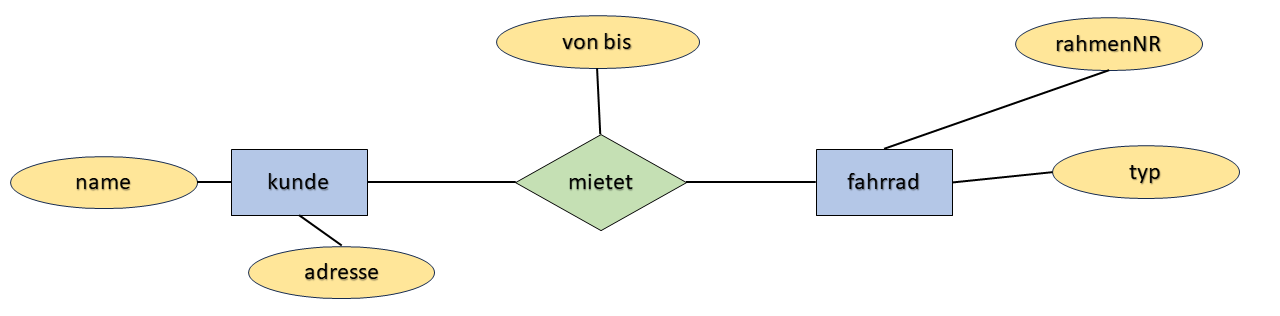
\includegraphics[width=\textwidth]{\pics/ERMFahrrad.png}
		\end{minipage}

		\item Ein befreundeter Autohändler bittet uns beim Aufbau einer Kundendatenbank zu helfen. Zuerst soll diese in einem ERM modelliert werden. Darin erscheinen sollen Kunde, Auto, Karosserietyp und Reifen. Ein Auto gehört dabei zu einem Kunden, ein Kunde kann aber mehrere Autos haben.

		\begin{minipage}{0.8\textwidth}
			\centering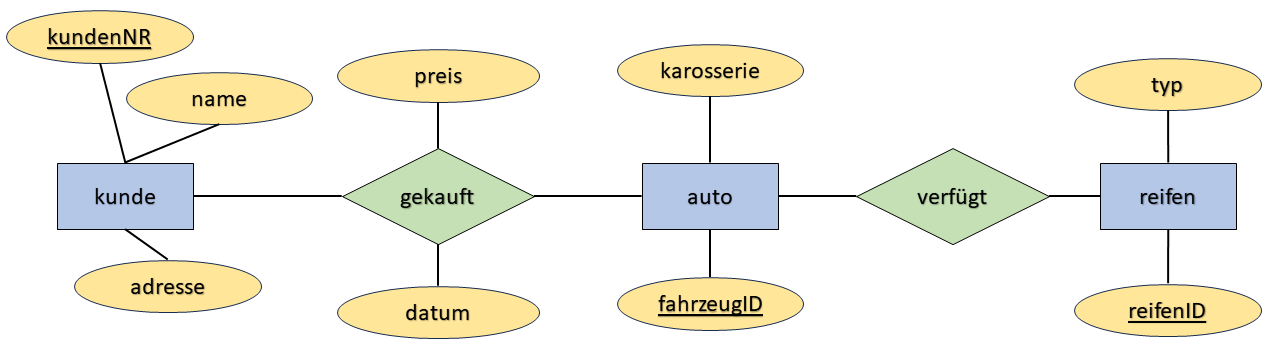
\includegraphics[width=\textwidth]{\pics/ERMAuto.png}
		\end{minipage}

		\item Ein DVD-Verleiher betreibt mehrere Filialen (id, strasse, plz), wo es jeweils mehrere Medien (DVDs, BluRays, Spiele) zu leihen gibt. Jeder Kunde kann nur einer Filiale zugeordnet sein. Jeder Kunde kann mehrere Medien ausleihen. Ein Mitarbeiter kann nur in einer Filiale arbeiten.

		\begin{minipage}{0.8\textwidth}
			\centering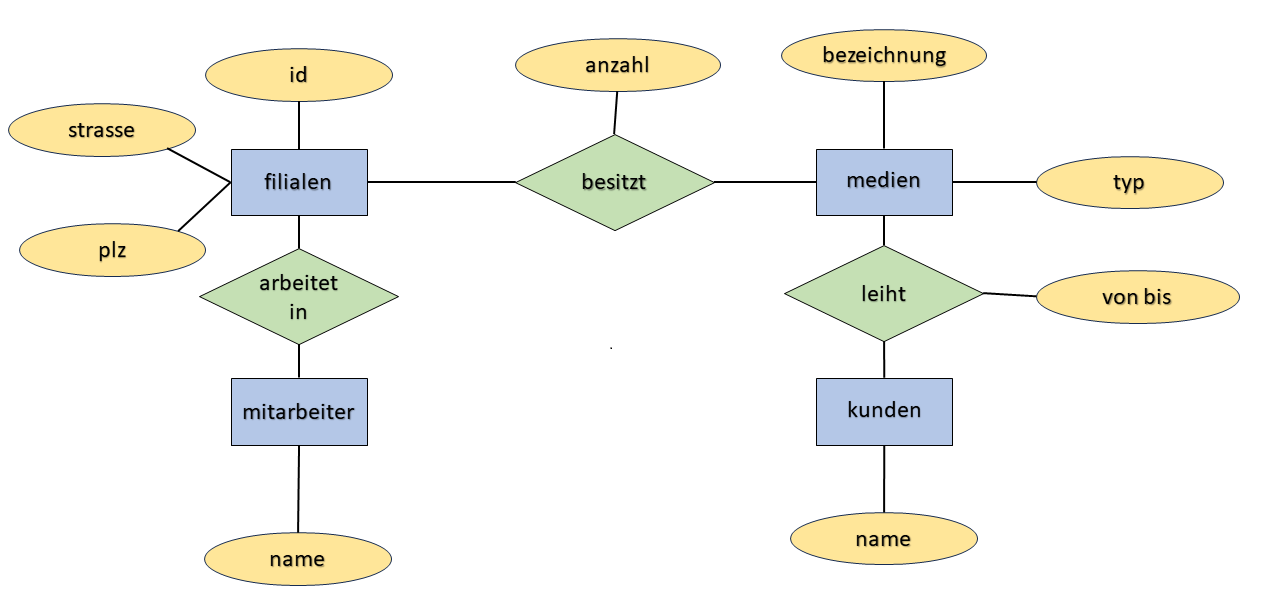
\includegraphics[width=\textwidth]{\pics/ERMDVDs.png}
		\end{minipage}
	\end{enumerate}
\end{Answer}

\subsection{Primärschlüssel und Kardinalitäten}
Der Primärschlüssel löst das Problem der Eindeutigkeit. Jede Entität, die auf der Datenbank gespeichert wird, muss eindeutig identifizierbar sein. Speichert z.B. eine Firma die Entität Kunde, so muss jeder Kunde eindeutig identifizierbar sein. Würde man als Attribute nur den Namen und Vornamen anhängen, so könnte man Diego Maradonna aus Bremen nicht von Diego Maradonna aus Stuttgart unterscheiden. Man kann natürlich einfach zusätzliche Attribute hinzufügen, wie z.B. das Geburtsdatum oder die Adresse, bis man sich sicher ist, dass es nicht zu Verwechslungen kommen kann, aber es gibt einen eleganteren Weg. Im Normalfall hängt man eine Nummer an (z.B. die Kundennummer), die für jede Entität eine andere sein muss. So kann man jede Entität eindeutig an Hand der Nummer identifizieren. Diego mit der Kundennummer 44445 ist dann eine andere Person als Diego mit der Kundennummer 85417. Diese Nummer bezeichnet man Primärschlüssel.
\begin{tcolorbox}[title=Primärschlüssel]
	Attribut, das eine Entität eindeutig identifizierbar macht. Im Normalfall eine laufende Nummer, d.h. bei jeder neu hinzukommenden Entität wird die Nummer einfach um eins größer gemacht. Der Primärschlüssel wird im ERM durch Unterstreichen kenntlich gemacht.
\end{tcolorbox}
\begin{tcolorbox}[title=Fremdschlüssel]
	Wird der Primärschlüssel eines Entitätstyps an einen anderen Entitätstyp als Attribut hinzugefügt, so bezeichnet man dieses Attribut als Fremdschlüssel.
\end{tcolorbox}
Die Kardinalität gehört zu Beziehungen und gibt an, wie viele Entitäten jeweils in Beziehung zueinander stehen können. Diesen Angaben schreibt man auf die Kanten zwischen den jeweiligen Entitätstypen und der Beziehung. Man unterscheidet im Wesentlichen folgende Kardinalitäten:

\begin{itemize}
	\item 1:1 Beziehung

	Jede Entität des einen Typs \(E_1\) ist maximal einer Entität des anderen Typs \(E_2\) zugeordnet und umgekehrt, z.B. hat jedes Land genau eine Hauptstadt und jede Hauptstadt liegt in genau einem Land.
	\begin{minipage}{0.8\textwidth}
		\centering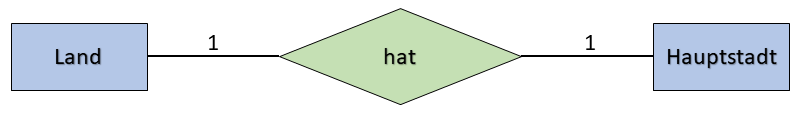
\includegraphics[width=\textwidth]{\pics/ERMBeziehungen11.png}
		Grafische Darstellung einer 1:1 Beziehung.
	\end{minipage}
	\item 1:N Beziehung

	Jeder Entität des einen Typs \(E_1\) sind beliebig viele Entitäten des zweiten Typs \(E_2\) zugeordnet. Umgekehrt sind jedoch jeder Entität vom Typ \(E_2\) maximal eine Entität vom Typ \(E_1\) zugeordnet, z.B. gehen mehrere Schüler in eine Klasse, umgekehrt geht aber ein einzelner Schüler in genau eine Klasse.

	\begin{minipage}{0.8\textwidth}
		\centering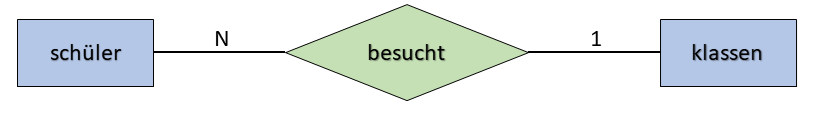
\includegraphics[width=\textwidth]{\pics/ERMBeziehungen1N.png}

		Grafische Darstellung einer 1:1 Beziehung.
	\end{minipage}
	\item N:M Beziehung

	Jeder Entität des einen Typs \(E_1\) sind beliebig viele Entitäten des zweiten Typs \(E_2\) zugeordnet und umgekehrt, z.B. kann ein Mitarbeiter an mehreren Projekten gleichzeitig arbeiten und umgekehrt können an einem Projekt mehrere Mitarbeiter gleichzeitig arbeiten.

	\begin{minipage}{0.8\textwidth}
		\centering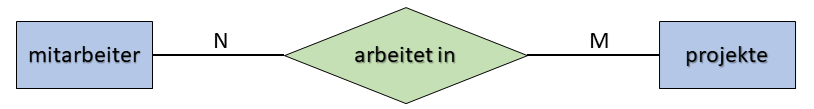
\includegraphics[width=\textwidth]{\pics/ERMBeziehungenNM.png}

		Grafische Darstellung einer 1:1 Beziehung.
	\end{minipage}
\end{itemize}

\subsection{Beispiel eines ERMs einer Firma}
Die Kunden einer Firma können Bestellungen aufgeben, die ein oder mehrere Artikel enthalten. Zu jeder Bestellung erhält der Kunde eine Rechnung. Für die Firma wichtig sind Name und Adresse der Kunden, das Datum der Bestellung, welche Artikel enthalten sind und wie teuer diese sind sowie der Betrag und das Fälligkeitsdatum der Rechnung:

\begin{minipage}{\textwidth}
	\centering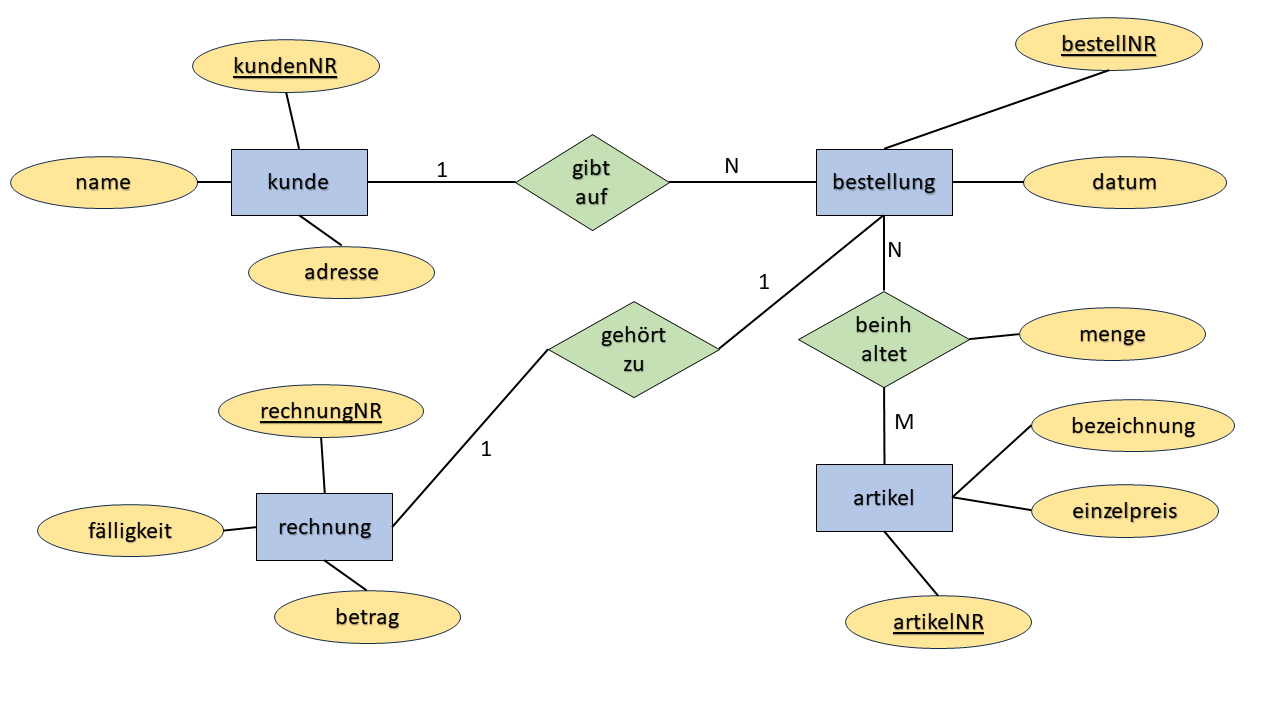
\includegraphics[width=\textwidth]{\pics/ERMFirmaEinfach.png}
\end{minipage}

Beispiel für ein ERM. Die Primärschlüssel sind jeweils unterstrichen. Die Kardinalitäten der Beziehungen ergeben sich aus folgenden Überlegungen:
\begin{itemize}
	\item Kunde zu Bestellung eine 1:N Beziehung. Ein Kunde kann mehrere Bestellungen aufgeben, aber jede Bestellung ist genau einem Kunden zugeordnet.
	\item Rechnung zu Bestellung eine 1:1 Beziehung. Hinter jeder Rechnung verbirgt sich genau eine Bestellung und zu jeder Bestellung wird genau eine Rechnung erstellt.
	\item Bestellung zu Artikel eine N:M Beziehung. In jeder Bestellung können mehrere (M verschiedene) Artikel vorkommen und umgekehrt kann ein Artikel in verschiedenen Bestellungen (N verschiedene) vorkommen.
\end{itemize}
\begin{Exercise}[title=Vervollständige die ERMs aus Aufgabe \ref{ERMErstellen1}. Jeder Entitätstyp muss einen Primärschlüssel haben und ergänze die Kardinalitäten., label=ERMErstellen2]
	\phantom{ }
\end{Exercise}
%%%%%%%%%%%%%%%%%%%%%%%%%%%%%%%%%%%%%%%%%%
\begin{Answer}[ref=ERMErstellen2]
	\begin{enumerate}
		\item Ein Fahrradverleih am Bodensee verleiht Damen-, Herren- und Kinderfahrräder. Dabei wird für jedes Fahrrad ein eigener Mietvertrag abgeschlossen. Eine Person kann mehrere Fahrräder mieten. Der Fahrradverleih möchte eine Datenbank aufbauen. Helfen Sie dabei.

		\begin{minipage}{0.8\textwidth}
			\centering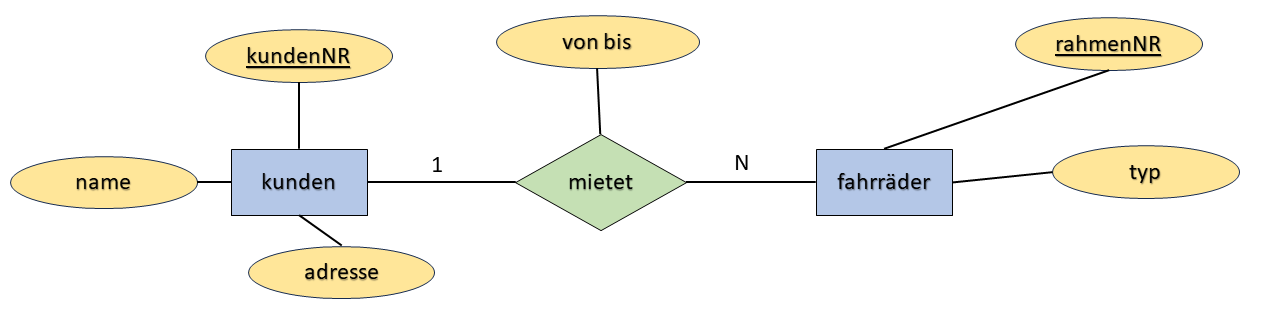
\includegraphics[width=\textwidth]{\pics/ERMFahrradvoll.png}
		\end{minipage}
		\item Ein befreundeter Autohändler bittet uns beim Aufbau einer Kundendatenbank zu helfen. Zuerst soll diese in einem ERM modelliert werden. Darin erscheinen sollen Kunde, Auto, Karosserietyp und Reifen. Ein Auto gehört dabei zu einem Kunden, ein Kunde kann aber mehrere Autos haben.

		\begin{minipage}{0.8\textwidth}
			\centering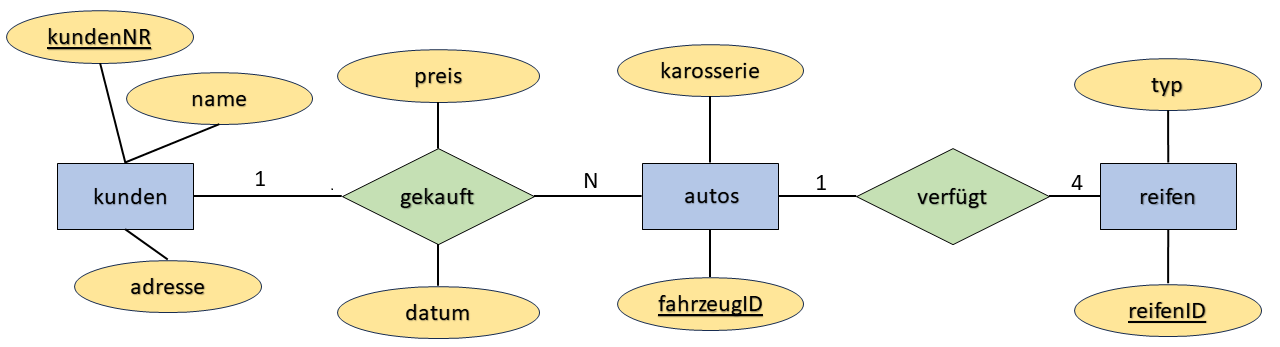
\includegraphics[width=\textwidth]{\pics/ERMAutovoll.png}
		\end{minipage}
		\item Ein DVD-Verleiher betreibt mehrere Filialen (id, strasse, plz), wo es jeweils mehrere Medien (DVDs, BluRays, Spiele) zu leihen gibt. Jeder Kunde kann nur einer Filiale zugeordnet sein. Jeder Kunde kann mehrere Medien ausleihen. Ein Mitarbeiter kann nur in einer Filiale arbeiten.

		\begin{minipage}{0.8\textwidth}
			\centering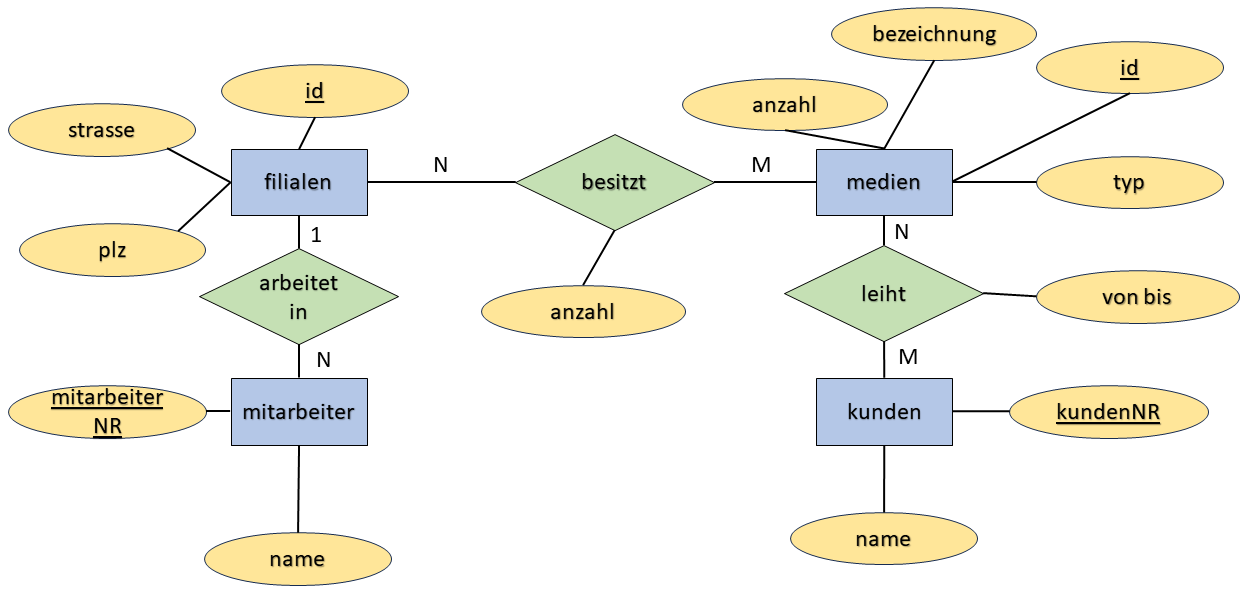
\includegraphics[width=\textwidth]{\pics/ERMDVDsvoll.png}
		\end{minipage}
	\end{enumerate}
\end{Answer}

\begin{Exercise}[title=Erstelle ein ERM., label=ERMErstellen3]
	In der Oberstufe eines Gymnasiums wird nicht mehr in Klassen, sondern in Kursen unterrichtet. Sie erhalten von der Schulleitung den Auftrag, eine Kursverwaltung mittels des Entity-Relationship-Modells zu modellieren. Mit Hilfe dieser Kursverwaltung soll festgehalten werden, welche Schüler welche Kurse besuchen. Als Schülerdaten soll neben dem Vornamen und Nachnamen der Schüler auch die individuelle Schülernummer, das Geburtsdatum, Geschlecht sowie die Postadresse festgehalten	werden. Jeder Kurs hat eine eigene Kursnummer. Außerdem sind der Kurstyp (5stündig / 2stündig), das Fach (z.B. D, M, E, …) und die Jahrgangsstufe (K1 / K2) zu speichern. In dem neuen System sollen auch die Fehlstunden und Kursnoten jedes Schülers dokumentiert werden. Jeder Kurs ist einem Lehrer zugeordnet. Als lehrerspezifische Daten sollen dessen Vor- und Nachname, das Kürzel und seine Fächer (max. 2) mit in das Kursverwaltungsprogramm aufgenommen werden.
\end{Exercise}
\begin{Answer}[ref=ERMErstellen3]
	In der Oberstufe eines Gymnasiums wird nicht mehr in Klassen, sondern in Kursen unterrichtet. Sie erhalten von der Schulleitung den Auftrag, eine Kursverwaltung mittels des Entity-Relationship-Modells zu modellieren. Mit Hilfe dieser Kursverwaltung soll festgehalten werden, welche Schüler welche Kurse besuchen. Als Schülerdaten soll neben dem Vornamen und Nachnamen der Schüler auch die individuelle Schülernummer, das Geburtsdatum, Geschlecht sowie die Postadresse festgehalten werden. Jeder Kurs hat eine eigene Kursnummer. Außerdem sind der Kurstyp (5stündig / 2stündig), das Fach (z.B. D, M, E, …) und die Jahrgangsstufe (K1 / K2) zu speichern. In dem neuen System sollen auch die Fehlstunden und Kursnoten jedes Schülers dokumentiert werden. Jeder Kurs ist einem Lehrer zugeordnet. Als lehrerspezifische Daten sollen dessen Vor- und Nachname, das Kürzel und seine Fächer (max. 2) mit in das Kursverwaltungsprogramm aufgenommen werden.

	\begin{minipage}{\textwidth}
		\centering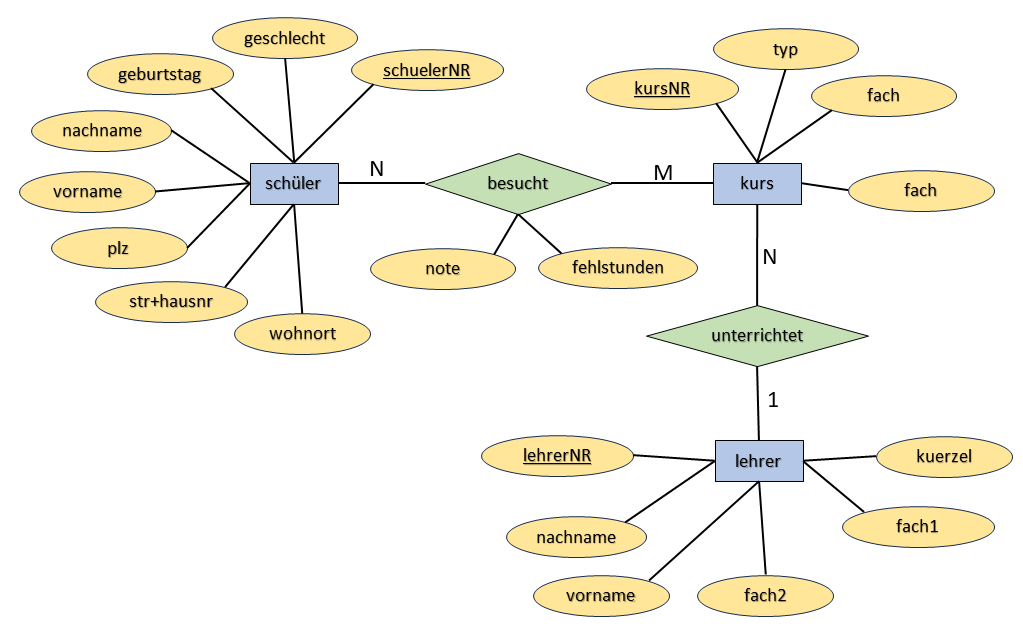
\includegraphics[width=\textwidth]{\pics/ERMOberstufe.png}
	\end{minipage}
\end{Answer}
